\documentclass[11pt]{article}
\usepackage{amssymb}
\usepackage{amsmath}
\usepackage{centernot}
\usepackage{amsfonts}
\usepackage{eurosym}
\usepackage{geometry}
\usepackage{ulem}
\usepackage{graphicx}
\usepackage{tikz}
\usepackage{rotating}
\usepackage{caption}
\usepackage{color}
\usepackage{setspace}
\usepackage{sectsty}
\usepackage{comment}
\usepackage{footmisc}
\usepackage[inline]{enumitem}
\usepackage{caption}
\usepackage{natbib}
\usepackage{pdflscape}
\usepackage{subfigure}
\usepackage{array}
\usepackage{titling}
\usepackage{multirow}
\usepackage{diagbox}
\usepackage{dcolumn}
\usepackage{makecell}
\usepackage[hidelinks]{hyperref}
\hypersetup{unicode = true}

\normalem

\onehalfspacing
\newtheorem{theorem}{Theorem}
\newtheorem{corollary}[theorem]{Corollary}
\newtheorem{proposition}{Proposition}
\newenvironment{proof}[1][Proof]{\noindent\textbf{#1.}}{\ \rule{0.5em}{0.5em}}

\newtheorem{hyp}{Hypothesis}
\newtheorem{subhyp}{Hypothesis}[hyp]
\renewcommand{\thesubhyp}{\thehyp\alph{subhyp}}
% \renewcommand{\labelenumi}{H.\arabic{enumi}.} % Redefine new labels for hyp
\newcommand{\T}{\rule{0pt}{2.6ex}}            % Top strut
\newcommand{\B}{\rule[-1.2ex]{0pt}{0pt}}      % Bottom strut
\newcommand{\red}[1]{{\color{red} #1}}
\newcommand{\blue}[1]{{\color{blue} #1}}
\newcommand{\ci}{\perp\!\!\!\perp}
\newcommand{\nci}{\centernot{\ci}}
\newcommand{\subtitle}[1]{\posttitle{\par\end{center}\begin{center}\large#1\end{center}\vskip0.5em}}
\newcommand{\refp}[1]{(\ref{#1})}

\newcolumntype{L}[1]{>{\raggedright\let\newline\\arraybackslash\hspace{0pt}}m{#1}}
\newcolumntype{C}[1]{>{\centering\let\newline\\arraybackslash\hspace{0pt}}m{#1}}
\newcolumntype{R}[1]{>{\raggedleft\let\newline\\arraybackslash\hspace{0pt}}m{#1}}

\geometry{left=1.0in,right=1.0in,top=1.0in,bottom=1.0in}

\begin{document}

\begin{titlepage}
\title{Three Essays on Sanctions of Politicians in Brazil}
\subtitle{A proposal submitted in partial fulfillment of the requirements for the Degree of Doctor of Philosophy in Public Policy}
\author{Andre Assumpcao\thanks{PhD Student, Department of Public Policy, The University of North Carolina at Chapel Hill. Contact details: \href{mailto:aassumpcao@unc.edu}{\textcolor{blue}{aassumpcao@unc.edu}}}}

\maketitle

\begin{abstract}
\noindent This dissertation project will investigate the relationship between legal sanctions and politics in Brazil. In the first paper, I look at the effect of convictions for electoral infractions on electoral performance in four municipal elections between 2004 and 2016. The second paper tests whether State Court judges significantly rule in favor of politicians involved in small claim court cases. Finally, the last paper investigates whether active and passive transparency simultaneously improve government performance and increase the number of legal sanctions for government wrongdoing. These papers contribute significantly to the literature in political science, economics, and law by exploring the relationship between legal sanctions and local political dynamics in developing countries. In addition, I also contribute new data sources in the form of judicial decisions and innovative identification strategies using institutional features of Brazilian electoral and judicial systems. \\
\vspace{0in} \\
\noindent\textbf{Keywords:} political economy of development; electoral politics; judicial politics; transparency; economics of crime. \\
\vspace{0in}
\bigskip

\end{abstract}

\setcounter{page}{0}

\thispagestyle{empty}

\end{titlepage}

\clearpage

\section{Active and Passive Transparency in Brazilian Municipalities} \label{sec:paper3}

\subsection{Introduction} \label{subsec:introduction_paper3}

Institutional scholarship often claims that government transparency is a key factor for good governance and economic development \citep{KaufmannGovernanceMatters1999,BoRothsteinGoodGovernance2012}. When governments make their business public, they allow for the scrutiny and oversight of actions taken by elected officials and civil servants. In many countries, for instance, citizens can check the use of public resources by accessing expense reports filled by politicians and, if unhappy, demand proper use of government funds. Under these conditions, transparency creates an accountability mechanism aligning interests of agents and principals and further supporting economic and social progress. In recent debates about the impact of institutions on development, however, there is an increasing push for more granular understanding of these accountability mechanisms. Investigations on the endogeneity of institutions and their strength \citep{AcemogluChapterInstitutionsFundamental2005,LevitskyVariationInstitutionalStrength2009,DalBoInstitutionsBehaviorExperimental2010} are becoming more widespread and this project contributes to this scholarship as the first account of the simultaneous effects of \emph{active} and \emph{passive} transparency on government performance.

There are many studies looking at active and passive transparency separately. The former can be understood \emph{as any action initiated by government, or its partners, releasing information about government business}, of which top-down monitoring is the most important mechanism. Using experimental evidence from Indonesia, \citet{OlkenMonitoringCorruptionEvidence2007c} shows that delivering top-down audits of road construction projects with certainty reduces the amount of missing funds by eight percentage points, while grassroots community initiatives have no effect on the misallocation of public resources. \citet{FerrazExposingCorruptPoliticians2008b} investigate whether the release of corruption information via audits impacts the electoral performance of incumbent mayors in the Brazilian municipal elections of 2004. They find that stronger corruption allegations (as measured by the level of corruption revealed in the audit reports) significantly reduced the chances of incumbent reelection by as much as seven percentage points. In the presence of a local AM radio station, the impact increases to a 23 percentage point hit to the probability of reelection of incumbent mayors. \citet{BobonisMonitoringCorruptiblePoliticians2016} document a 67 percent reduction in corruption when municipalities in Puerto Rico undergo their timely audits before election period, and corroborates the evidence that top-down monitoring consistently prevents misallocation of resources.

The monitoring effect on corruption is present even when accountability comes from media coverage. \citet{CampanteIsolatedCapitalCities2014} show that isolated U.S.~state capitals have higher corruption levels, as measured by federal convictions for corruption-related crimes, due to the lower concentration of population and newspapers in and around their geographical area. This media monitoring effect does not only impact criminal behavior, such as corruption, but also non-criminal behavior, such as day-to-day political work. \citet{SnyderJrPressCoveragePolitical2010} use the geographical intersections of media markets and U.S.~congressional districts to isolate the effect of media coverage on political behavior. They find that representatives from districts where media coverage is larger are more aligned with their constituents' preferences, more likely to participate in congressional hearings, and to serve in committees directly relevant to their constituents. Though these studies  are conducted at different periods and across different countries, they jointly point to the same positive effect of active transparency on government accountability.

Passive transparency, on the other hand, has only recently become a topic of academic interest, so much so that it does not have a widely-accepted definition yet. To that end, I define it \emph{as any action initiated by government, or its partners, in which information is made available but released only upon request}. The key difference to active transparency is the information release component. In actuality, passive transparency has mostly taken the form of freedom of information acts (FOIAs). FOIAs constitute dormant accountability measures which are activated when there is an explicit request from the public, the media, or any other non-governmental agent. In one of the earlier analysis of freedom of information policies, \citet{EscalerasFreedominformationacts2010} find that passive transparency does not reduce corruption; in fact, in developing nations, their evidence is that implementing FOIAs actually \emph{increases} corruption. \citet{CostaFreedomInformationLaws2013} corroborates these findings with micro-level data from the World Bank Business Environment and Enterprise Performance Survey, where she shows that after the adoption of FOI laws firms are eight to 12 percentage points more likely to perceive corruption as an obstacle to business. These studies, however, rely on corruption perception indexes and thus are susceptible to two simultaneous measurement errors: the increase in corruption could come from (i) FOIAs detecting more of otherwise uncovered corruption in \citet{EscalerasFreedominformationacts2010}, leading to (ii) firms perceiving more corruption in \citet{CostaFreedomInformationLaws2013}. Both cases are compatible with unchanged (or lower) levels of corruption. The results in \citet{CordisSunshineDisinfectantEffect2014} are more aligned with the expected relationship between passive transparency and corruption: using the same corruption (objective) measure of \citet{CampanteIsolatedCapitalCities2014}, federal convictions for corruption-related crimes, they find that U.S.~states switching from weak to strong FOIA institutions experience twice as many corruption detection and conviction cases.

To my knowledge, this is the first study bringing together active and passive transparency. At first, analyzing the joint effect of transparency might seem uninteresting. If separately these policies improve governance, either by looking at corruption or political behavior, and are both expressions of government accountability, then it is intuitive to conclude that both favor good governance and performance. A more nuanced reasoning, however, reveals interesting puzzling questions. In a world where government resources are scarce, authorities might perceive them as competing policies and choose the implementation of one over the other. As such, any analysis that directly compares the effect of each alternative is of great policy value. In addition, if we allow for heterogeneous behavior of individuals working in government, we can expect different reactions to the implementation of either policy, e.g.~they might fear audits more than FOIA requests. Finally, there are a number of recent studies looking at whether better informed voters can ensure better governance practices \citep{PandeCaninformedvoters2011,WintersLackingInformationCondoning2013,ChongDoesCorruptionInformation2015,Weitz-ShapiroCanCitizensDiscern2017}. An open question remains as to which type of transparency produces the most credible information for holding politicians and bureaucrats accountable for their actions.

I take advantage of an unique policy environment in Brazil to answer these questions. Between 2003 and 2015, the Office of the Comptroller-General (CGU) implemented a random audit program investigating the use of federal resources by municipalities across Brazil to implement local public policies. This program provides exogenous variation in active transparency for a random sample of municipalities during this period. In 2012, however, Brazil also enacted its Freedom of Information Act, known  \emph{in portuguese} as LAI, establishing channels of information release across all government levels. By overlaying random audits and LAI across municipalities over time, I artificially create a two-by-two factorial experiment where municipalities fall into one of four treatment arms: (i) control (municipalities not audited before LAI); (ii) passive transparency (municipalities not audited after LAI); (iii) active transparency (municipalities audited before LAI); (iv) active and passive transparency (municipalities audited after LAI). I then compare the effect of these treatments on government performance and sanctions applied to government, politicians, and civil servants charged with wrongdoing between 2006 and 2018.

Besides the random audit policy, CGU also established a program in 2015 called \emph{Transparent Brazil Scale} (EBT), which measures the implementation of the freedom of information act across a random sample of municipalities via submission of homogeneous information requests to local governments. To the same extent as the corruption findings published in CGU reports,\footnote{As extensively discussed in \citet{FerrazExposingCorruptPoliticians2008b,FerrazElectoralAccountabilityCorruption2011a,BrolloPoliticalResourceCurse2013,ZamboniAuditRiskRent2018,AvisGovernmentAuditsReduce2018}.} the data collected in the EBT program forms an unbiased, objective measure of information quality when FOIAs are enacted -- precisely speaking to the credible information literature. Thus, using the outcomes from both CGU programs, I take one step further and provide estimates of the cross-effect of transparency, i.e.~the effect of active transparency on information quality and the effect of passive transparency on misallocation of resources.

Preliminary results indicates significant cross-effects. For audited municipalities, passive transparency reduces corruption by 13.2 percent but increases acts of mismanagement by 45.9 percent. This result suggests that passive transparency does not unconditionally improve government performance; rather, it reduces corruption at the expense of mismanagement. In the period after the implementation of LAI (post-2012), being audited actually reduces the quality of information by (5.2 percentage points) but has no effect on time taken to respond back to information requests. This is not an entirely unexpected result, since officials might feel more pressured to respond to information requests after being audited but compromise information quality in the process. The effects of both treatments on the probability of sanctions and the adoption of an urban development plan are not statistically significant, indicating little additional contribution of one transparency program when another is in place. I discuss this further in the results section.

The remaining of this paper is organized as follows: in section \ref{subsec:background_paper3}, I discuss the institutional design that allows for the causal identification of both active and passive transparency effects; section \ref{subsec:data_paper3} presents the data used in this project; section \ref{subsec:theory_paper3} suggests the theoretical mechanisms and hypotheses of the impact of various types of transparency on government performance; section \ref{subsec:methods_paper3} outlines the empirical strategy yielding the results in section \ref{subsec:results_paper3}; finally, section \ref{subsec:conclusion_paper3} lays out the steps necessary for the conclusion of this project.

\subsection{Institutional Background} \label{subsec:background_paper3}

The Office of the Comptroller-General (CGU) was established in 2003 to oversee the use of federal resources across the executive branch. Its mission involved investigating and guaranteeing proper use of resources not only across the federal executive, but also across all levels of executive government -- states and municipalities included. Over time, its attributions have expanded from a purely monitoring function to rule-making and even the imposition of legal sanctions on state and municipal governments, public officials, and private parties contracted by Brazilian government. Since its inception, CGU has been the most important anti-corruption agency in the country and, despite political change, it has maintained its high-profile status as an autonomous oversight agency within the federal government.

CGU is responsible for a number of transparency programs. It processes freedom of information requests at the federal executive level, it hosts annual conferences on fighting corruption, it works jointly with other legal authorities (Federal Policy and the Office of the Prosecutor-General) to conduct investigations on misuse of public resources, it publishes civil servant wages, just to name a few of its roles. One of its most recognized programs is the random audit of municipalities, which begun in 2003 and ended in 2015.\footnote{The program still exists today but, instead of randomly selecting and auditing municipalities, CGU uses an internal risk score model to assign audits to municipalities most at risk of corruption.} This program consisted of a short visit, generally a week or two long, to a municipality for the investigation of the use of federal resources in public services. The central CGU office provided state teams with a list of inspection orders, covering transfers from the federal level to municipalities in the previous three to four years, and the state team would check this list against the records provided by municipal officials. After the visit, auditors summarized their findings in a report which was then made available on CGU's website and forwarded to the all prosecuting authorities, such as the Federal Police, and local legislative branches, e.g.~city councils and state legislative bodies.

The program has been successful since the beginning. In 2004, CGU fed the Federal Police evidence of a corruption scheme covering over 100 procurement contracts for the purchase of emergency vehicles in 119 municipalities between 2000 and 2002, with an estimated loss of \$7 million (in 2002 dollars). In addition, the program design has made it a prolific source of academic research. CGU randomly selected a certain number of municipalities in each state, along with the (monthly) federal lottery draws, and assigned teams of independent, highly-qualified bureaucrats to scrutinize all expenditures made by municipalities under policy programs. CGU officials are tenured civil servants who have been approved in national competitive exams and whose income is both independent of their audit findings and higher than the national average for professionals of same qualification. Thus, not only the random audit program is an excellent source of unbiased, objective measures of municipal corruption for the period between 2003 and 2015 in Brazil, but also constitutes an exogenous shock of active transparency imposed on a sample of municipalities since 2003.

The second institutional feature making Brazil the perfect case for this research project is the passage of its freedom of information act (LAI), approved by the Brazilian Congress in 2011 but coming into force in May 2012. The law required that all government branches, levels, and its affiliated agencies set-up systems of access to public information. Its provisions are similar to that of other FOIAs across the world: all information is public unless expressed and justified by the agency responsible; no agency can charge for use of government data; any individual or company, national or foreign, can file a request for data access. The nationwide scope, the immediate effect, and the standardized, mandatory rules established by LAI make it an exogenous shock of passive transparency across Brazil in May 2012.

While the random audit program both creates an exogenous shock of active transparency and a rich dataset of objective measures of corruption, the same is not true of LAI -- which only imposes the passive transparency shock. Thus, I create the objects measures of information quality using another program managed by CGU, called \emph{Transparent Brazil Scale} (EBT). The EBT program started in 2015 and it created a national ranking of the quality of freedom of information systems across municipalities and states based on a set of standardized objective criteria. These criteria form a very detailed, 20-page evaluation guide on many aspects in LAI ranging from a check on whether the local government has a functioning website to the actual submission of four information requests. What is even more interesting is that EBT is also applied on a random sample of Brazilian municipalities; CGU has a detailed sampling strategy available online for two out of three rounds of EBT,\footnote{I have submitted a LAI request to CGU to obtain the sampling strategy for the first round, which is also a random draw on about 9\% of all municipalities in each state of Brazil.} where they explain how municipalities are sampled and how their scores are calculated. Thus, EBT also provides an unbiased, objective measure of information quality useful in answering the research questions in this proposal.

\subsection{Data} \label{subsec:data_paper3}

The data come from various sources and spans over multiple years (2003-2018). I construct a repeated cross-section database of Brazilian municipalities with corruption, information, performance, and sanction outcomes. The variables of interest are audit (active) treatment, LAI (passive) treatment, and both (active and passive transparency). I supplement all analyses with municipal covariates and year of observation indicator variables.

Corruption outcomes come from the random audit program run by CGU until 2015. For transparency purposes, I use the same dataset as \citet{AvisGovernmentAuditsReduce2018}, which is public available as a response to a freedom of information request on CGU's website. It contains all inspection orders in municipalities randomly selected for audits since 2006, which is when CGU developed their standardized coding of corruption and mismanagement infractions. The corruption, mismanagement, and number of irregularities outcomes are the same as \citet{AvisGovernmentAuditsReduce2018}, i.e.~the (logged) number of infractions of each type. The level of observation is the municipality-lottery pair, so there are 1,084 observations for 1,011 unique municipalities in this dataset.\footnote{This reflects the fact that some municipalities have been randomly selected to inspection more than once.}

The data on transparency information comes from the EBT program. Specifically, I use four information requests sent to municipalities in the evaluation of three EBT rounds in 2015, 2016, 2017. These requests measured the quality of information on two dimensions: (i) whether the municipality reported back in the time mandated by LAI; (ii) whether the information provided was accurate. These four requests covered four policy areas: health, education, social development, and transparency. For the time outcome, I compute whether the municipality has responded to any of the four requests within the deadline. For the accuracy dimension, I compute whether the municipality has provided correct answers to any of the four requests. It is important to point out that CGU submitted information requests on policy programs that are crafted at the federal level but delivered at the local level; therefore, for these programs, CGU maintains a federal record of implementation that can be compared to responses provided by local governments so as to construct a perfect measure of information accuracy. There are 2,327 unique municipalities (level of analysis) in this sample. When I join this data with audit reports, there are 3,287 total observations (2,830 municipalities) receiving at least one of the transparency treatments.

Next, the third source of data is the Brazilian National Statistics Office (IBGE). It produces a statistical profile of municipalities every two or three years, from which I extract the performance outcome in this study. According to the Brazilian Constitution, all municipalities with population above 20,000 are required to have a municipal urban development plan (MUDP). These plans lay out land use regulations and zoning laws that support structured spatial growth of municipalities. Since crafting such a plan needs inputs from all areas of local government, they are good proxies of performance as they are only as good as the people who put them together. In addition, though mandated by law, MUDPs have an expiry date and are enacted into law by negotiation between city councils and mayors, so it is not unusual to find a number of municipalities that do not have a valid urban development plan at any point in time. Therefore, I build a dataset of MUDP adoption for all waves of the statistical profile issued by IBGE and match them to audit and EBT municipalities in this study.

Finally, I create the sanction outcome from three datasets of agencies with investigative authority in Brazil. The Federal Police and CGU have public data on corruption crackdown operations carried out across the country since 2003 (also used in \citet{AvisGovernmentAuditsReduce2018}). I use their dataset to track municipalities that have had one of these operations as mandated by judicial rulings. The second dataset comes from CGU and reports all independent CGU operations which aimed at seizing evidence as part of an ongoing corruption investigation at the federal level. I again match the municipalities in this sample that were targeted by these operations. Finally, I use a dataset on nationwide convictions for misuse of public resources maintained by the National Council of Justice. It compiles information from all state court systems on politicians or bureaucrats who were convicted for violations to the law preventing misconduct in public office (Law 8,429/92). Again, I match municipalities in our sample and compute if they have had at least one conviction for breach of law 8,426/92. The final sanction outcome is a binary variable for a municipality-year pair if any of three sanctions have been applied to a municipal government over the time under analysis.

Descriptive statistics are reported in table \ref{tab:descriptivestats3}, where I display covariates used in this analysis. These municipal characteristics come from the Brazil Census of 2010 and control for variation in municipal conditions that could bias treatment results.

% latex table generated in R 3.5.1 by xtable 1.8-2 package
% Wed Dec  5 11:33:15 2018
\begin{table}[!htbp]
\centering
\caption{Descriptive Statistics by Treatment Condition}
\label{tab:descriptivestats3}
\scriptsize
\begin{tabular}{@{\extracolsep{-4pt}}l@{\extracolsep{-3pt}}ccccccccc}
\hline
\hline
& \multicolumn{2}{c}{\emph{Active}} & & \multicolumn{2}{c}{\emph{Passive}} & & \multicolumn{2}{c}{\emph{Active and Passive}} \T \\
& \multicolumn{2}{c}{\emph{Transparency}} & & \multicolumn{2}{c}{\emph{Transparency}} & & \multicolumn{2}{c}{\emph{Transparency}} \B \\
\cline{2-3} \cline{5-6} \cline{8-9}
& Control & Treatment & Diff. & Control & Treatment & Diff. & Control & Treatment & Diff. \T \B \\
& (1) & (2) & (3) & (1) & (2) & (3) & (1) & (2) & (3) \B \\
\hline
Share Urban (Pop.)                   & 0.632 & 0.626 & 0.006   & 0.625 & 0.631 & -0.007  & 0.630 & 0.629 & 0.002   \T \\
                                     &       &       & (0.411) &       &       & (0.405) &       &       & (0.890)    \\
Share Female (Pop.)                  & 0.505 & 0.505 & 0.000   & 0.505 & 0.505 & -0.001  & 0.505 & 0.506 & -0.001     \\
                                     &       &       & (0.463) &       &       & (0.178) &       &       & (0.513)    \\
Illiteracy Rate                      & 0.170 & 0.181 & -0.010  & 0.179 & 0.171 & 0.007   & 0.172 & 0.185 & -0.013     \\
                                     &       &       & (0.001) &       &       & (0.039) &       &       & (0.013)    \\
Income Per Capita (ln)               & 9.150 & 9.046 & 0.104   & 9.052 & 9.140 & -0.089  & 9.132 & 9.030 & 0.102      \\
                                     &       &       & (0.000) &       &       & (0.000) &       &       & (0.004)    \\
Gini Coefficient                     & 0.510 & 0.512 & -0.002  & 0.512 & 0.510 & 0.003   & 0.510 & 0.511 & -0.001     \\
                                     &       &       & (0.250) &       &       & (0.269) &       &       & (0.767)    \\
Human Development Index \vspace{1pt} & 0.653 & 0.645 & 0.008   & 0.645 & 0.652 & -0.007  & 0.652 & 0.644 & 0.008      \\
                                     &       &       & (0.000) &       &       & (0.007) &       &       & (0.030)    \\
Share Poor (Pop.)                    & 0.249 & 0.270 & -0.021  & 0.270 & 0.251 & 0.019   & 0.253 & 0.270 & -0.017     \\
                                     &       &       & (0.000) &       &       & (0.003) &       &       & (0.081)    \\
Presence of AM Radio                 & 0.204 & 0.199 & 0.005   & 0.203 & 0.203 & 0.000   & 0.204 & 0.189 & 0.015      \\
                                     &       &       & (0.685) &       &       & (0.990) &       &       & (0.466)    \\
Presence of Health Council           & 0.759 & 0.776 & -0.017  & 0.767 & 0.762 & 0.004   & 0.761 & 0.801 & -0.040     \\
                                     &       &       & (0.203) &       &       & (0.781) &       &       & (0.067)    \\
Presence of Ed. Council              & 0.973 & 0.968 & 0.005   & 0.971 & 0.972 & -0.001  & 0.973 & 0.959 & 0.014      \\
                                     &       &       & (0.326) &       &       & (0.868) &       &       & (0.203)    \\
Seat of Judiciary Branch             & 0.500 & 0.501 & -0.001  & 0.486 & 0.503 & -0.017  & 0.498 & 0.538 & -0.041     \\
                                     &       &       & (0.968) &       &       & (0.346) &       &       & (0.133) \B \\
\hline
\emph{N} & 4,177 & 1,326 & & 960 & 4,543 & & 5,137 & 366 & \T \B \\
\hline
\hline
\multicolumn{10}{p{.95\textwidth}}{\emph{Note:} This table displays means for all observations in each treatment arm against all other. Thus, the sum of observations is larger than the total sample size (5,503). Columns (1)-(3) are the means for the control group, the treatment group, and difference across means; \emph{p}-values are displayed in parentheses.}
\end{tabular}
\end{table}


According to table \ref{tab:descriptivestats3}, differences across groups are small and mostly concentrated in income-related covariates (illiteracy rates, income per capita, Gini coefficient, Human Development Index, share of poor population). These differences are mostly due to potential differences present in 2010, when these covariates are measured, that could have likely decreased over time. Besides, there are small differences in the sampling strategy and sample size between the two programs. While the random audits were limited to 180 municipalities per year, at most, EBT selected over 1,000 municipalities to form its ranking in each round between 2015 and 2017. Also, random audits were constrained to municipalities under 450,000-500,000 residents whereas EBT sampled municipalities across the the whole distribution of population size. In any case, I estimate all regressions controlling for these covariates to reduce the potential for bias in our parameters of interest.

Though there are overlapping treatment arms, the most important limitation of this study is the lack of information and corruption outcomes for all observations in the sample. Since the outcomes are produced by the same programs that assign treatments to municipalities, I can only measure such outcomes following the subgroups in table \ref{tab:treatmentarms}.

\begin{table}[!htbp]
  \caption{\label{tab:percentreversed}Observations by Transparency Condition}
  \centering
  \scriptsize
  \begin{tabular}{@{\extracolsep{12pt}}r|rr|r}
    \hline
    \hline
    & \multicolumn{2}{c}{\emph{Passive}} \vline & \T \B \\
    \multicolumn{1}{r}{\emph{Active}} \vline & Pre-LAI & Post-LAI & Total \T \B \\
    \hline
    Not Audited & -   & 4,177 & 4,177 \T \B \\
    Audited     & 960 & 277   & 1,187 \T \B \\
    \hline
    Total       & 960 & 4,404 & 5,364 \T \B \\
    \hline
    \hline
  \end{tabular}
\end{table}

Corruption outcomes are only available for observations in row ``Audited'' while information outcomes are only measured for observations for column ``Post-LAI.'' While I use these subgroups under either treatment for measuring cross-effects, I want to investigate further the joint effect of either treatment on performance and sanctions. To that end, I need to draw a random sample of Brazilian municipalities that have not been audited prior to 2012 so that I include them as the control group in this project. I lay out this sampling strategy in the following section.

\subsubsection{Sampling Strategy} \label{subsec:sampling_paper3}

This project is not a social experiment according to standard industry practices. The researcher is not manipulating the environment, has not chosen the outcomes of interest, and has no pre-analysis plan to bind the research methods and hypotheses \emph{ex-ante}. Its unique design, however, is in many ways similar to an experimental study allowing for causal identification of different transparency effects. Audit treatment participants are randomly selected from the universe of Brazilian municipalities both before and after the implementation of LAI, so I can mimic a combined randomized control trial (audits) plus difference-in-differences (LAI) design to isolate the causal effect of each transparency type.

I have identified two relevant outcomes for this research design: government performance and sanctions imposed on local governments, politicians, and bureaucrats as the result of police and judicial investigations. I already have the panel with outcomes for all Brazilian municipalities over the period 2003 and 2018. The remaining step to create the artificial two-by-two experimental design is the random draw of the control group. Following best practices in the experimental literature, I am aiming at a five percentage point minimum detectable effect size with 90 percent power and five percent alpha. The power calculation is represented by figure \ref{fig:power} below and indicates a sample size of 4,203 municipalities, which means the control group should have at least 916 observations. Thus, in the final version of this project, I will include this subsample in the analysis in section \ref{subsec:results_paper3}. Unfortunately, I cannot balance the number of observations across all treatment conditions since I am using two interventions previously implemented by government.
\clearpage
\begin{figure}
\centering
\caption{Power Calculation for Sampling Strategy}
\label{fig:power}
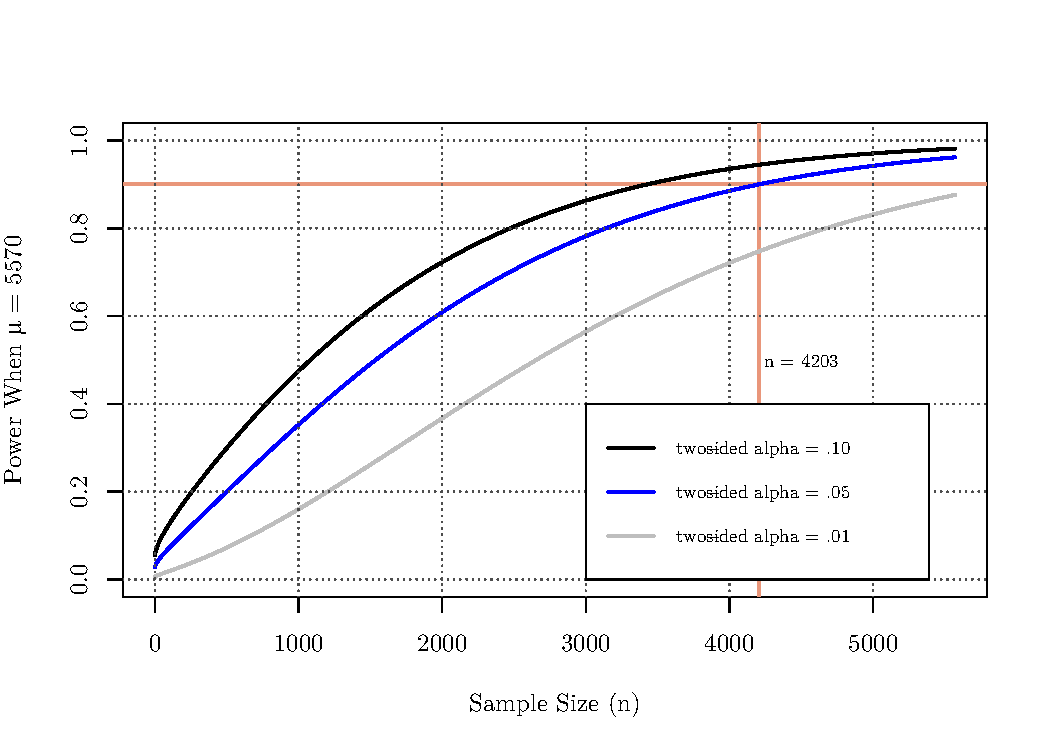
\includegraphics[trim = {0 0 0 2cm}, clip, scale = .75]{power.pdf}
\end{figure}

The final sampling strategy follows closely that of audit lotteries, the reasoning being that LAI treatment is uniform across municipalities but only  outcomes are collected randomly (as discussed in section \ref{subsec:background_paper3}). The strata then are the six years and 26 states for which audit lotteries were conducted before 2012. The random draw and methodology will form an appendix to the final version of this project.

\subsection{Theory and Hypotheses} \label{subsec:theory_paper3}

In this paper, I investigate the relationship between transparency and government performance. I suggest breaking down transparency into two finer subgroups, active and passive transparency, and look at two main outcomes that most closely align to similar studies in the literature.

\subsubsection{Active Transparency} \label{subsubsec:theory1_paper3}

Active transparency speaks to the studies looking at ways to prevent wrongdoing in government, mostly described by either corruption or misallocation of resources. \citet{BeckerCrimePunishmentEconomic1968,BeckerLawEnforcementMalfeasance1974,Rose-AckermanEconomicsCorruption1975} pioneered this field of research by suggesting that criminal behavior can be described by individual cost-benefit calculations, that government should choose an optimal level of law enforcement which depends on enforcement cost functions, and that corruption incentives depend on market structure in the provision of goods and services being contracted by government. Audits are attempts at uncovering wrongdoing, e.g.~increasing the probability of crime detection, that come at a cost of setting up teams, sending them out to municipalities, producing audit reports, and everything else involved in the investigations. Though these municipal corruption markets are likely decentralized, I can expect municipal governments to exert significant market power as a result of the low penetration of firms and markets in development settings. The efficiency gains of preventing corruption are likely to be large and thus we can expect better government performance in the presence of active transparency.

\paragraph{Performance Hypothesis (H1a).} \emph{A municipal government that has experienced an active transparency intervention (audits) should see an improvement in government performance (measured by the adoption of urban development plans).}\\

Increasing the detection of wrongdoing should be followed by the imposition of more sanctions, which comes from prosecuting authorities having more cases, or more evidence, available. The reasoning is straightforward. Prosecutors have a fixed endowment of time to pursue various criminal cases (income effect zero), see an inflow of government malfeasance cases or evidence (relative price of prosecuting such cases falls), and substitute out other cases for cases involving misuse of public office (substitution effect is positive). This relationship is captured in hypothesis 2a.

\paragraph{Sanction Hypothesis (H2a).} \emph{The imposition of active transparency initiatives (audits) should be followed by an increase in sanctions imposed for government wrongdoing (measured by the likelihood of being targeted in operations seizing evidence and judicial convictions).} \\

I lastly expect that audits positively impact information quality. When local governments welcome a team of auditors and have to go through their program records in order to answer inspector questions, it is likely that it will learn from the experience and improve information storage in response to increased scrutiny. As a result, both the time it takes to release information and the accuracy with which government data is communicated would see improvements after a CGU audit has taken place. Hypothesis 3 summarizes this reasoning.

\paragraph{Information Hypothesis (H3).} \emph{In the presence of active transparency measures (audits), governments are likely to improve the quality of information release (measured by the time to respond to freedom of information requests and the accuracy of the information in the responses).}

\subsubsection{Passive Transparency} \label{subsubsec:theory2_paper3}

Passive transparency can also be seen as a measure to increase detection and prosecution of government crimes. However, it has not been as explored as other monitoring initiatives have, so its theoretical underpinnings are less widely understood.

The first important question is whether any type of transparency is inherently positive (a discussion first held in \citet{PratWrongKindTransparency2005}). In the above case, the release of information concerning corruption or poor allocation of resources is beneficial, since both actions are detrimental to social welfare. Principals want less of both. This might not be true of passive transparency. Governments would scramble to organize their files and make sure all information is available at the expense of its core responsibilities. If, eventually, these data are not requested by anyone outside government, or if data are requested but there are no wrongdoings, then passive transparency has unequivocally consumed resources and has not produced social benefits.\footnote{The case where there are benefits of organizing information for active transparency is difference in at least two dimensions. First, the former case is primarily concerned with the use of resources instead of all data on government activities. The benefits of investigating an correcting use of funds is much more clear than that of making all municipal normative acts public; second, in cases where public administration is sound, it is likely that benefits of transparency have been exhausted or are close to zero as we can reasonably assume that the returns to transparency are decreasing in scale.} Mostly likely, social welfare improves where administration problems abound, i.e.~when public officials are not highly-skilled, or when there is an active civil society interested in government affairs. Moreover, if the implementation of freedom of information acts simultaneously reduces corruption and increases the detection of government malfeasance, these effects could largely offset each other and show no significant effect of passive transparency on government efficiency, as rightly suggested in \citet{CordisSunshineDisinfectantEffect2014}. As a result, I cautiously construct hypotheses H1b.

\paragraph{Performance Hypothesis (H1b).} \emph{A municipal government that has experienced an passive transparency intervention (post-LAI) should see an improvement in government performance (measured by the adoption of urban development plans) of smaller magnitude when compared to active transparency.}\\

Since active transparency is more focused and drives more attention to politicians and bureaucrats alike, I expect it to be a stronger driver of performance. Local governments in Brazil are generally less effective and usually attract less-skilled professionals, as discussed in [...], so I would still expect a positive but attenuated effect of LAI implementation. For the sanctions hypothesis, however, I expect a positive effect, the reason being that passive transparency is supports the application of sanctions on governments and officials since it expands the toolkit available to prosecuting authorities to collect data.

\paragraph{Sanction Hypothesis (H2b).} \emph{The imposition of passive transparency initiatives should be followed by an increase in sanctions imposed for government wrongdoing (measured by the likelihood of being targeted in operations seizing evidence and judicial convictions).} \\

The impact on corruption should also be straightforward. For municipalities that have experienced an audit in the past, that know the implications of being audited and the legal risks of inspection findings for governments, politicians, and officials, the adoption of LAI should be an additional source of concern that have a strong discipling effect on the use of resources. Hypothesis 4 summarizes this relationship.

\paragraph{Corruption Hypothesis (H4).} \emph{In the presence of passive transparency initiatives (LAI), governments shift away from corruption.}

Clearly, I cannot know with certainty whether corruption has reduced because corrupt officials have decided to steer clear from such practices or because they have become more skilled at hiding their behavior. In the preliminary analysis section (\ref{subsec:results_paper3}), I suggest looking at other audit outcomes to try and answer this question.

\subsubsection{Active and Passive Transparency} \label{subsubsec:theory3_paper3}

The double treatment is available for the performance and sanction outcomes. As discussed in previous sections, however, I unfortunately do not observe corruption and information outcomes for all municipalities in this sample. This is a direct limitation of the exogenous shocks and outcome measurements created by audit and LAI interventions. Nevertheless, the evidence I present in cross-effect analysis are also new to the literature and contribute to the relevance of this project.

I first claim that double treatment effects will be smaller than single treatment effects combined. In other words, I am suggesting that the interaction between active and passive monitoring produces decreasing returns to scale. When a municipality has experienced one type of transparency, the other would just marginally add to improving social welfare.

\paragraph{Performance Hypothesis (H1).} \emph{A municipal government experiencing double transparency treatment should see a proportionally smaller performance improvement than the sum of the two independent treatment effects.}

\paragraph{Sanction Hypothesis (H2).} \emph{A municipal government experiencing double transparency treatment should see a proportionally smaller sanction improvement than the sum of the two independent treatment effects.} \\

The decreasing returns come from various sources. First, both treatments might reveal the same information used for prosecuting wrongdoing or create the same incentives for setting up a urban development plan. Second, governments, politicians, and bureaucrats might not perceive the second transparency intervention as concerning as the first. Once problems, or sound governance, have been revealed in the first wave of transparency, there is a smaller reputation effect of confirming further good or bad governance. In fact, there is no way of knowing whether there will be a second information release action since establishing freedom of information channels does not imply the release of public documents (which is true for audits). Therefore, it seems straightforward to conclude that double treatment has decreasing returns to scale. In sum, table displays the relationships in this section.
\clearpage
\begin{table}[!htbp]
  \caption{Hypotheses Table by Treatment Condition}
  \label{tab:hypotheses3}
  \centering
  \scriptsize
  \begin{tabular}{l|p{1.5cm}|p{1.5cm}|p{1.5cm}}
  \hline
  \hline
                   & \multicolumn{1}{c}{Double}& \multicolumn{1}{c}{Active}& \multicolumn{1}{c}{Passive} \T \B \\
  \hline
  (H1) Performance & \multicolumn{1}{c}{$+$}   & \multicolumn{1}{c}{$+$}   & \multicolumn{1}{c}{$+$}     \T \B \\
  (H2) Sanction    & \multicolumn{1}{c}{$+$}   & \multicolumn{1}{c}{$+$}   & \multicolumn{1}{c}{$+$}     \T \B \\
  (H3) Information & \multicolumn{1}{c}{}      & \multicolumn{1}{c}{$+$}   & \multicolumn{1}{c}{$+$}     \T \B \\
  (H4) Corruption  & \multicolumn{1}{c}{}      & \multicolumn{1}{c}{$-$}   & \multicolumn{1}{c}{$-$}     \T \B \\
  \hline
  \hline
  \end{tabular}
\end{table}

\subsection{Empirical Strategy} \label{subsec:methods_paper3}

I estimate the effect of both types of transparency on repeated cross-sections of municipal observations in Brazil between 2006 and 2017. Municipal characteristics are observed in the 2010 Census. Municipalities belong to one of the four quadrants in table \ref{tab:treatmentarms}. Since CGU audits are randomly assigned over the period of 2006 and 2015, I can compare municipalities audited before and after the introduction of the freedom of information act in 2012 to identify the causal effect of passive transparency on corruption. \citet{AvisGovernmentAuditsReduce2018} use a similar sample and find that the number of irregularities found in these audit reports is relatively stable across municipalities, suggesting that there is no heterogeneity in audit quality over time.
\begin{equation} \label{eq:eq1_paper3}
  y_{i} = \alpha + \rho \cdot \text{LAI} + X \beta + \sum \lambda_{k} + \varepsilon_{i}
\end{equation}

In equation \refp{eq:eq1_paper3}, $y_{i}$ is the audit outcome of interest, either the (logged) number of (i) acts of corruption, (ii) mismanagement, or (iii) any irregularity for municipality $i$. Treatment condition is captured by $\text{LAI}$, which becomes one for municipalities audited in or after 2012, and $\rho$ is the causal effect of passive transparency on $y_{i}$. The matrix of municipal characteristics is represented by $X$ and $\lambda_{k}$ are $k$lottery fixed-effects to absorb up any time-invariant component of the stochastic error term $\varepsilon_{i}$. This equation is symmetric for information outcomes. Since these outcomes are only observed for a random sample of municipalities participating in the EBT, and the audits are also randomly assigned to municipalities, I have unbiased outcomes, sample selection, and treatment assignment yielding unbiased estimates of active transparency on information quality.
\begin{equation} \label{eq:eq2_paper3}
  y_{i} = \alpha + \rho \cdot \text{audit} + X \beta + \sum \lambda_{k} + \varepsilon_{i}
\end{equation}

The dependent variables $y_{i}$ are whether CGU's freedom of information requested are responded within the mandated legal deadline and whether the information provided was accurate. Treatment condition is being audited ($audit$) and the causal parameter of interest is $\rho$. $X$ is the matrix of municipal characteristics and $\lambda_{f}$ are the $k$ year of data collection fixed-effects to also control for time-invariant effects in the error term.

Effects on performance and sanction outcomes are estimated using regression equation \refp{eq:eq3_paper3}, a standard difference-in-differences equation. Performance and sanction are binary dependent variables turning on when the municipality either adopts a urban development plan or is the targeted of a sanctioning operation by CGU, the Federal Police, or the Judiciary.
\begin{equation} \label{eq:eq3_paper3}
  y_{i} = \alpha + \rho_{1} \cdot \text{LAI} + \rho_{2} \cdot \text{audit} + \gamma \cdot \text{LAI} \times \text{audit} + X \beta + \sum \lambda_{k} + \varepsilon_{i}
\end{equation}

\subsection{Preliminary Results} \label{subsec:results_paper3}


\begin{table}[!htbp] \centering
  \caption{The Effect of Active Transparency on Information Requests}
  \label{tab:transparency2}
\scriptsize
\begin{tabular}{@{\extracolsep{5pt}}lcccc}
\\[-1.8ex]\hline
\hline \\[-1.8ex]
& \multicolumn{4}{c}{Outcomes:} \T \B \\
\cline{2-5}
 & \multicolumn{2}{c}{FOI Request (time)} & \multicolumn{2}{c}{FOI Request (accuracy)} \T \B \\
\\[-1.8ex] & \multicolumn{1}{c}{(1)} & \multicolumn{1}{c}{(2)} & \multicolumn{1}{c}{(3)} & \multicolumn{1}{c}{(4)} \B \\
\hline \\[-1.8ex]
 Active Transparency & $-.073^{***}$ & $-.050^{*}$ & $-.085^{***}$ & $-.063^{**}$ \\
                     & (.028) & (.026) & (.029) & (.027) \\
                     & & & & \\
\hline \\[-1.8ex]
Municipal Controls & \multicolumn{1}{c}{-} & \multicolumn{1}{c}{Yes} & \multicolumn{1}{c}{-} & \multicolumn{1}{c}{Yes} \\
Year Fixed-Effects & \multicolumn{1}{c}{-} & \multicolumn{1}{c}{Yes} & \multicolumn{1}{c}{-} & \multicolumn{1}{c}{Yes} \\
\hline \\[-1.8ex]
Observations & \multicolumn{1}{c}{4,404} & \multicolumn{1}{c}{4,404} & \multicolumn{1}{c}{4,404} & \multicolumn{1}{c}{4,404} \\
R$^{2}$ & \multicolumn{1}{c}{.002} & \multicolumn{1}{c}{.122} & \multicolumn{1}{c}{.002} & \multicolumn{1}{c}{.123} \\
Adjusted R$^{2}$ & \multicolumn{1}{c}{.001} & \multicolumn{1}{c}{.119} & \multicolumn{1}{c}{.002} & \multicolumn{1}{c}{.120} \\
\hline
\hline \\[-1.8ex]
\multicolumn{5}{p{.6\textwidth}}{\emph{Note:} This table displays the regressions measuring the effect of active transparency (being audited by a team of officials from the Office of the Comptroller-General -- \emph{CGU}) on information requests for a random sample of municipalities across Brazil participating in the \emph{Transparent Brazil} program. For each outcome, I display two regressions including and excluding municipal controls and year fixed-effects. The variable of interest is whether the municipality was audited by CGU after 2012. Clustered (at the municipal level) robust standard errors are in parentheses. $^{*}$p$<$0.1; $^{**}$p$<$0.05; $^{***}$p$<$0.01.}\\
\end{tabular}
\end{table}



\begin{table}[!htbp] \centering
\caption{The Effect of Passive Transparency on Corruption}
\label{tab:corruption1}
\scriptsize
\begin{tabular}{@{\extracolsep{-2pt}}lD{.}{.}{-3} D{.}{.}{-3} D{.}{.}{-3} D{.}{.}{-3} D{.}{.}{-3} D{.}{.}{-3} }
\\[-1.8ex]\hline
\hline \\[-1.8ex]
& \multicolumn{2}{c}{Acts of Corruption (ln)} & \multicolumn{2}{c}{Acts of Mismanagement (ln)} & \multicolumn{2}{c}{No. of Irregularities (ln)} \T \\
\\[-1.8ex] & \multicolumn{1}{c}{(1)} & \multicolumn{1}{c}{(2)} & \multicolumn{1}{c}{(3)} & \multicolumn{1}{c}{(4)} & \multicolumn{1}{c}{(5)} & \multicolumn{1}{c}{(6)} \B\\
\hline \\[-1.8ex]
Passive Transparency & -.132^{***} & -.142^{***} & .426^{***} & .429^{***} & -.098^{***} & -.106^{***} \\
										 & (.010) 		 & (.006) 		 & (.046) 		& (.046) 		 & (.008) 		 & (.005) \\
										 & & & & & & \\
\hline \\[-1.8ex]
Municipal Controls & \multicolumn{1}{c}{-} & \multicolumn{1}{c}{Yes} & \multicolumn{1}{c}{-} & \multicolumn{1}{c}{Yes} & \multicolumn{1}{c}{-} & \multicolumn{1}{c}{Yes} \\
\hline \\[-1.8ex]
Observations & \multicolumn{1}{c}{1,326} & \multicolumn{1}{c}{1,326} & \multicolumn{1}{c}{1,326} & \multicolumn{1}{c}{1,326} & \multicolumn{1}{c}{1,326} & \multicolumn{1}{c}{1,326} \\
R$^{2}$ & \multicolumn{1}{c}{.012} & \multicolumn{1}{c}{.258} & \multicolumn{1}{c}{.040} & \multicolumn{1}{c}{.052} & \multicolumn{1}{c}{.007} & \multicolumn{1}{c}{.227} \\
Adjusted R$^{2}$ & \multicolumn{1}{c}{.011} & \multicolumn{1}{c}{.251} & \multicolumn{1}{c}{.040} & \multicolumn{1}{c}{.044} & \multicolumn{1}{c}{.006} & \multicolumn{1}{c}{.220} \\
\hline
\hline \\[-1.8ex]
\textit{Note:}  & \multicolumn{6}{r}{$^{*}$p$<$0.1; $^{**}$p$<$0.05; $^{***}$p$<$0.01} \\
\end{tabular}
\end{table}



\begin{table}[!htbp] \centering
  \caption{The Effect of Active and Passive Transparency on Performance and Sanctions}
  \label{tab:performance3}
\scriptsize
\begin{tabular}{@{\extracolsep{.5cm}}lcccc}
\\[-1.8ex]\hline
\hline \\[-1.8ex]
& \multicolumn{4}{c}{Outcomes:} \T \B \\
\cline{2-5}
 & \multicolumn{2}{c}{MUDP Adoption} & \multicolumn{2}{c}{Official Sanctioned} \T \B \\
\\[-1.8ex] & \multicolumn{1}{c}{(1)} & \multicolumn{1}{c}{(2)} & \multicolumn{1}{c}{(3)} & \multicolumn{1}{c}{(4)}\\
\hline \\[-1.8ex]
 Active and Passive Transparency & $-.009$ & $-.026$ & \hspace{1pt} $.008$ & \hspace{1pt} $.010$ \\
                                 & (.034) & (.043) & (.013) & (.013) \\
                                 & & & & \\
\hline \\[-1.8ex]
Municipal Controls & \multicolumn{1}{c}{-} & \multicolumn{1}{c}{Yes} & \multicolumn{1}{c}{-} & \multicolumn{1}{c}{Yes} \\
Year Fixed-Effects & \multicolumn{1}{c}{-} & \multicolumn{1}{c}{Yes} & \multicolumn{1}{c}{-} & \multicolumn{1}{c}{Yes} \\
\hline \\[-1.8ex]
Observations & \multicolumn{1}{c}{5,364} & \multicolumn{1}{c}{5,364} & \multicolumn{1}{c}{5,364} & \multicolumn{1}{c}{5,364} \\
R$^{2}$ & \multicolumn{1}{c}{.000} & \multicolumn{1}{c}{.262} & \multicolumn{1}{c}{.000} & \multicolumn{1}{c}{.049} \\
Adjusted R$^{2}$ & \multicolumn{1}{c}{.000} & \multicolumn{1}{c}{.259} & \multicolumn{1}{c}{.000} & \multicolumn{1}{c}{.046} \\
\hline
\hline \\[-1.8ex]
\multicolumn{5}{p{.65\textwidth}}{\emph{Note:} This table displays the regressions measuring the effect of active and passive transparency (being audited by CGU after 2012) on the adoption of municipal development plans (MDP) and on sanctions imposed to politicians and bureaucrats for a sample of random municipalities selected for audits and participation in the \emph{Transparent Brazil} program. For each outcome, I display two regressions including and excluding municipal controls and year fixed-effects. The variable of interest is whether the municipality was audited by CGU after 2012. Clustered (at the municipal level) robust standard errors are in parentheses. $^{*}$p$<$0.1; $^{**}$p$<$0.05; $^{***}$p$<$0.01.}
\end{tabular}
\end{table}


\subsection{Further Development} \label{subsec:conclusion_paper3}

\clearpage

\setlength\bibsep{0pt}
\bibliographystyle{apalike}
\bibliography{/Users/aassumpcao/library.bib}

\end{document}